% The generic preamble
\documentclass[10pt,letterpaper,fleqn,titlepage]{article}

% Define packages to use
\usepackage{natbib}
\usepackage[dvips]{graphicx,color}
\usepackage{amsmath,amssymb}
\usepackage{bm}
\usepackage{caption}
\usepackage{xr}
\usepackage{ifthen}
\usepackage[dvipdfm,colorlinks,linkcolor=blue,citecolor=blue,urlcolor=blue]{hyperref}
\usepackage{fancybox}
\usepackage{textcomp}
\usepackage{alltt}
%\usepackage{floatflt}
%\usepackage{svn}


% Redefine default page
\setlength{\textheight}{9in}  % 1" above and below
\setlength{\textwidth}{6.75in}   % 0.5" left and right
\setlength{\oddsidemargin}{-0.25in}

% Redefine default paragraph
\setlength{\parindent}{0pt}
\setlength{\parskip}{1ex plus 0.5ex minus 0.2ex}

% Define caption width and default fonts
\setlength{\captionmargin}{0.5in}
\renewcommand{\captionfont}{\sffamily}
\renewcommand{\captionlabelfont}{\bfseries\sffamily}

% Define commands for super- and subscript in text mode
\newcommand{\superscript}[1]{\ensuremath{^\textrm{#1}}}
\newcommand{\subscript}[1]{\ensuremath{_\textrm{#1}}}

% Derived commands
\newcommand{\invcm}{\textrm{cm\superscript{-1}}}
\newcommand{\micron}{\ensuremath{\mu\textrm{m}}}

\newcommand{\df}{\ensuremath{\delta f}}
\newcommand{\Df}{\ensuremath{\Delta f}}
\newcommand{\dx}{\ensuremath{\delta x}}
\newcommand{\Dx}{\ensuremath{X_{max}}}
\newcommand{\Xeff}{\ensuremath{X_{eff}}}

\newcommand{\water}{\textrm{H\subscript{2}O}}
\newcommand{\carbondioxide}{\textrm{CO\subscript{2}}}
\newcommand{\ozone}{\textrm{O\subscript{3}}}

\newcommand{\taup}[1]{\ensuremath{\tau_{#1}}}
\newcommand{\efftaup}[1]{\ensuremath{\tau_{#1}^{*}}}

\newcommand{\textbfm}[1]{\boldmath\ensuremath{#1}\unboldmath}

\newcommand{\rb}[1]{\raisebox{1.5ex}[0pt]{#1}}

\newcommand{\f}[1]{\texttt{#1}}

% Define how equations are numbered
\numberwithin{equation}{section}
\numberwithin{figure}{section}
\numberwithin{table}{section}

% Define a command for title page author email footnote
\newcommand{\email}[1]
{%
  \renewcommand{\thefootnote}{\alph{footnote}}%
  \footnote{#1}
  \renewcommand{\thefootnote}{\arabic{footnote}}
}

% Define a command to print the Office Note subheading
\newcommand{\notesubheading}[1]
{%
  \ifthenelse{\equal{#1}{}}{}
  { {\Large\bfseries Office Note #1\par}%
    {\scriptsize \sc This is an unreviewed manuscript, primarily intended for informal}\\ 
    {\scriptsize \sc exchange of information among JCSDA researchers\par}%
  }
}

% Redefine the maketitle macro
\makeatletter
\def\docseries#1{\def\@docseries{#1}}
\def\docnumber#1{\def\@docnumber{#1}}
\renewcommand{\maketitle}
{%
  \thispagestyle{empty}
  \vspace*{1in}
  \begin{center}%
     \sffamily
     {\huge\bfseries Joint Center for Satellite Data Assimilation\par}%
     \notesubheading{\@docnumber}
  \end{center}
  \begin{flushleft}%
     \sffamily
     \vspace*{0.5in}
     {\Large\bfseries\ifthenelse{\equal{\@docseries}{}}{}{\@docseries: }\@title\par}%
     \medskip
     {\large\@author\par}%
     \medskip
     {\large\@date\par}%
     \bigskip\hrule\vspace*{2pc}%
  \end{flushleft}%
  \newpage
  \setcounter{footnote}{0}
}
\makeatother
\docseries{}
\docnumber{}


% Define a command for a DRAFT watermark
\usepackage{eso-pic}
\newcommand{\draftwatermark}
{
  \AddToShipoutPicture{%
    \definecolor{lightgray}{gray}{.85}
    \setlength{\unitlength}{1in}
    \put(2.5,3.5){%
      \rotatebox{45}{%
        \resizebox{4in}{1in}{%
          \textsf{\textcolor{lightgray}{DRAFT}}
        }
      }
    }
  }
}




% Derived commands
\newcommand{\microtesla}{\ensuremath{\mu\textrm{T}}}
\newcommand{\degree}{\ensuremath{^\circ}}

% Title info
\title{Validating Liebe and Rosenkranz Simulations of SSMIS channels 19-21}
\author{David Neil Groff\email{david.groff@noaa.gov}\\JCSDA/EMC/SAIC\\[0.25in]
        Paul van Delst\email{paul.vandelst@noaa.gov}\\JCSDA/EMC/SAIC\\[0.25in]
        Yong Han\email{yong.han@noaa.gov}\\JCSDA/NESDIS/STAR}
\date{February, 2008}
\docnumber{6}
\docseries{CRTM}


%-------------------------------------------------------------------------------
%                            Ze document begins...
%-------------------------------------------------------------------------------
\begin{document}
\maketitle

\section{Introduction}
%=====================
In the presence of a magnetic field transitional absorption/emission lines of molecules are split into multiple closely spaced lines. This splitting is known as the Zeeman effect and it is related to the broadening of absorption lines relative to an unsplit state. The magnitude of the broadening/splitting is directly related to the magnetic field strength ($B$).

The Special Sensor Microwave Imager/Sounder (SSMIS) upper atmosphere sounding channels 19-21 are significantly affected by Zeeman splitting, because the passbands for these channels are centered on or near O\subscript{2} rotational absorption lines \cite{Han2007}. 

SSMIS channels 19 and 20 each have two passbands that are centered on unsplit O\subscript{2} rotational transition lines; whereas SSMIS channel 21 has 4 passbands that are very close to and offset symetrically from unsplit O\subscript{2} rotational absorption lines. Therefore, broadening of absorption lines associated with an increasing $B$ decreases the altitudes where the weighting functions peak for channels 19 and 20 and increases the altitude where the weighting function peaks for channel 21. The magnitude of the Zeeman splitting impact on SSMIS measurements is also dependent on the angle between the magnetic field and the viewing direction, $\theta_{b}$, because the component of radiation received from each of the split lines depends on $\theta_{b}$. As $\theta_{b}$ increases abosrption becomes increasingly asymmetric about the position of unsplit line centers. This acts to decrease the component of absorption attributed to the unsplit line center. For SSMIS channels 19 and 20 the altitudes where the weighting functions peak decreases, because the passbands for thes channels are centered on unsplit O\subscript{2} absorption lines. In the case of SSMIS channel 21 the relationship is less obvious, but the passbands for this channel are sufficiently close to unsplit line centers such that the peak weighting function altitude for this channel decreases as $\theta_{b}$ increases. The relationship between $B$, $\theta_{b}$ and the weighting functions for channels 19-21 is depicted in Figure \ref{fig:Weight_Function}.
\begin{figure}[htp]
  \centering{}
  \includegraphics[scale=0.6]{./graphics/Weight_Function.eps}
  \caption{(a) Weighting functions calculated with $B$=23\microtesla{} (solid lines) and $B$=63\microtesla{} (dashed lines) at cos$\theta_{b}$=0.9 and (b) with cos$\theta_{b}$=0 (solid lines) and cos$\theta_{b}$=1 (dashed lines) at $B$=60\microtesla{} for a standard US atmosphere.   (Where $\theta_{b}$ is the angle between the view direction and the geomagnetic field). Taken from \cite{Han2007}.}
  \label{fig:Weight_Function}
\end{figure}

The weighting functions for SSMIS channels 19 and 20 peak at altitudes in the mesosphere where the lapse rate is normally negative. Therefore, as $\theta_{b}$ and/or $B$ increase, brightness temperatures for channels 19 and 20 should increase assuming the sensor zenith angle and atmosphere are fixed. For channel 21 the relationship between $B$, $\theta_{b}$ and brightness temperature is less obvious because the weighting function for this channel peaks near the boundary of the mesosphere and stratosphere.
 


\section{Purpose} 
%================
In this report the Liebe93 RT model \cite{Liebe1993} with a Zeeman approximation included and the Liebe93 without a Zeeman approximation included (hereafter referred to as "Liebe93 Zeeman" [LZ] and "Liebe93 no Zeeman" LNZ respectively) \cite{Liebe1993} are validated against a fast model (hereafter referred to as "true Zeeman" [TZ]) that accounts for the Zeeman effect and has been shown to significantly reduce observation versus model brightness temperature (BT) residuals for high peaking SSMIS channels 19-21 \cite{Han2007}. The primary motivation for this work is to determine to what extent the differences between the TZ and LNZ/RNZ models are consistent with the Zeeman splitting impact described in the introduction.  


\section{Description of TZ Model}
%================================
%\subsection{TZ Model}

The TZ model was trained with the Rosenkranz and Staelin [1988] model \cite{Rosenkranz1998}. The training data set was obtained for zenith angles between 51$\degree$ and 54$\degree$, 11 magnetic field strengths ranging from 20\microtesla to 60\microtesla and six view directions with respect to the magnetic field ranging from 0$\degree$ to 90$\degree$\cite{Han2007}. Inputs for this model are layer temperature, cosine($\theta_{b}$) and $B$. Brightness temperatures for channels 19-24 are output for zenith angles of approximately 52.5$\degree$ that are representative of the peak weighting function altitudes and an SSMIS scan angle of 45$\degree$. To confirm that the model was being used appropriately example results provided by the developers were reproduced and are displayed in Table \ref{tab:example_res}. 
\begin{table}[htp]
  \centering
  \begin{tabular}{c c}
    Example & Reproduced \\
    \hline 
    234.43 & 243.4348 \\
    202.05 & 202.0462 \\
    259.02 & 259.0163 \\
    266.30 & 266.2962 \\
    251.89 & 251.8929 \\
    236.08 & 236.0784 \\    
  \end{tabular}
  \caption{Table showing that example results have been reproduced}
  \label{tab:example_res}
\end{table}
 
In Figure \ref{fig:TZ_results} the impact of Zeeman splitting as a function of the geomagnetic field strength is plotted for 11 different $\theta_{b}$ values. The calculations were performed for a set of six U.S. standard atmospheres. For the plots in Figure \ref{fig:TZ_results} all differences/offsets are relative to BT's calculated at a base geomagnetic field strength of 20\microtesla. At all view geometries with respect to the geomagnetic field the absolute magnitudes of the differences/offsets for channels 19 and 20 are similar to the absolute magnitude of the difference/offset for channel 21. As expected the magnitude of Zeeman splitting impact on brightness temperatures for SSMIS channels 19-21 increases as $B$ increases for all view geometries plotted. 
\begin{figure}[htp]
  \centering{}
  \includegraphics[scale=0.8]{./graphics/TZ_results.eps}
  \caption{Brightness temperatures as a function of the geomagnetic field strength for 11 view geometries with respect to the geomagnetic field.}
  \label{fig:TZ_results}
\end{figure}


\section{Rosenkranz Versus Liebe}
%================================
Figures \ref{fig:Rosenkranz_V_Liebe} and \ref{fig:Rosenkranz_V_Liebe_RMS} are representative of the mean and RMS differences between LNZ and RNZ brightness temperatures for 48 University of Maryland Baltimore College (UMBC) profiles. Brightness temperatures calculated from LNZ and RNZ transmittances agree to within 0.02K for SSMIS channels 19-21. The RMS differences are less than 0.03K for channels 19-21. These differences are small compared to the absolute impact of Zeeman splitting for $B$=0.4\microtesla{} or greater as shown in figure \ref{fig:TZ_results}. Therefore, it is reasonable to consider the RNZ and LNZ simulations for SSMIS channels 19-21 interchangeable when making comparisons to models that account for the Zeeman effect (i.e TZ/LZ). 

\begin{figure}[htp]
  \centering{}
  \includegraphics[scale=0.8]{./graphics/Rosenkranz_V_Liebe.eps}
  \caption{Mean brightness temperature differences between the Rosenkranz and Liebe models which do not account for Zeeman splitting.}
  \label{fig:Rosenkranz_V_Liebe}
\end{figure}

\begin{figure}[htp]
  \centering{}
  \includegraphics[scale=0.8]{./graphics/Rosenkranz_V_Liebe_RMS.eps}
  \caption{RMS brightness temperature differences between the Rosenkranz and Liebe models which do not account for Zeeman splitting.}
  \label{fig:Rosenkranz_V_Liebe_RMS}
\end{figure}


\section{LNZ Versus LZ}
%======================
The LZ model assumes a magnetic field of 60\microtesla. Figure \ref{fig:Liebe_Comparison} is representative of mean BT differences between LZ and LNZ for six U.S. standard atmospheres. 
 
\begin{figure}[htp]
  \centering{}
  \includegraphics[scale=0.8]{./graphics/Liebe_Comparison.eps}
  \caption{Mean brightness temperature differences between the Liebe93 model with a Zeeman approximation and the Liebe93 model without a Zeeman approximation}
  \label{fig:Liebe_Comparison}
\end{figure}
 
The sign of the differences for SSMIS channels 19-21 are consistent with Figure \ref{fig:TZ_results} and with the discussion in the introduction section of this report. However, the magnitude of the differences for channels 19 and 20 are more than a factor of two smaller than the magnitude of the difference for channel 21. This result is not consistent with the TZ calculations shown in Figure \ref{fig:TZ_results}.

  
\section{TZ Versus LNZ}
%======================
Figure \ref{fig:TZ_Versus_LNZ} shows brightness temperature differences between TZ and LNZ at 23\microtesla{} and 60\microtesla{}. The sign of the differences and the absolute magnitude of the differences in \ref{fig:TZ_Versus_LNZ} are not consistent with relative changes/offsets shown in the \ref{fig:TZ_results} plots. The Figure \ref{fig:TZ_results} offsets are relative to a calculation that accounts for the Zeeman Effect given a magnetic field of 20\microtesla{}. As the magnetic field is increased the TZ model BT's are more similar to the LNZ BT's for channels 19 and 20. Furthermore, as $B$ increases the BT's for channels 19 and 20 increase. These features are not consistent with the arguments/discussion in the introduction section.
   
\begin{figure}[htp]
  \centering{}
  \includegraphics[scale=0.8]{./graphics/TZ_Versus_LNZ.eps}
  \caption{Mean differences between a fast RT model that accounts for the Zeeman Effect and a reference "Zeeman turned off"
   model. The differences were calculated for magnetic fields of 23\microtesla{} and 60\microtesla{}}
  \label{fig:TZ_Versus_LNZ}
\end{figure}


\section{Conclusion}
%===================
The TZ model is used as a reference for validating LNZ, LZ and RNZ simulations, because it has been shown to reduce observation versus model BT residuals. Brightness temperature simulations for SSMIS channels 19-21 using the TZ model are consistent with a reasoned argument for the impact of Zeeman splitting provided in the introduction. Brightness temperature differences between the LNZ and TZ simulations decrease as B increases. Furthermore, the BT's for channels 19 and 20 increase as $B$ increases. These features are not consistent with the discussion in the introduction section of this report.


% The references section
%=======================
\bibliographystyle{plain}
\bibliography{bibliography}	

\end{document}
